% HW 2 report - ES 1402, Helmholtz-resonator bottle tuned by water level
% plot_matlab.png (from analyze_plunger.m) must be in the same folder.

\documentclass[12pt]{article}

\usepackage[utf8]{inputenc}
\usepackage{geometry}
\geometry{letterpaper, margin=1in}
\usepackage{setspace}
\usepackage{titlesec}
\usepackage{enumitem}
\usepackage{array}
\usepackage{booktabs}

\titlespacing*{\section}{0pt}{1.0em}{0.4em}
\titlespacing*{\subsection}{0pt}{0.8em}{0.3em}

\setstretch{1.3}
\usepackage{hyperref}
\hypersetup{
    colorlinks=true,
    linkcolor=blue,
    filecolor=blue,
    urlcolor=blue,
    citecolor=blue,
    pdfborder={0 0 0}
}
\usepackage{xcolor}
\usepackage{tcolorbox}
\usepackage{amsmath}
\usepackage{amssymb}
\usepackage{amsfonts}
\usepackage{graphicx}
\usepackage{fancyhdr}
\pagestyle{fancy}
\fancyhf{}
\fancyfoot[C]{\thepage}

% \newcommand{\hwNumber}{\#2}
\newcommand{\hwTitle}{Tuning a single note}

\begin{document}

%% ------------------------- Cover page -------------------------
\begin{center}
    \vspace*{2cm}
    \textbf{Vanderbilt University \\}
    \textbf{School of Engineering \\}
    \vfill
    \textbf{ES 1402-13 \\}
    \textbf{Dr. Bellan\\}
    \textbf{Fall 2026-2027\\}
    \textbf{\today \\}
    \textbf{HW 2: \hwTitle \\}
    \vfill
    \textbf{Youssef Nassar \\}
    (Student ID: nassary) \\
    \vfill
\end{center}

\thispagestyle{empty}
\newpage
\pagenumbering{arabic}

\fancyhead[L]{\textbf{Vanderbilt University}}
\fancyhead[C]{\textbf{\hwTitle\ \hwNumber}}
\fancyhead[R]{\textbf{ES 1402}}

%% ------------------------- Page 2: setup and data -------------------------
\section*{Instrument and Setup}

\begin{itemize}[itemsep=0.6em]
    \item \textbf{Instrument:} Helmholtz-resonator bottle, a 355 mL Aquafina plastic bottle (brim volume 393 mL) tuned by water level; a 60 mL syringe measures the water removed.
    \item \textbf{Tuned quantity (X):} water removed $x$ in mL, equivalent to air volume added; $x = 0$ is the starting fill (air volume 50 mL), and I measured $x = 0$ to $30$ mL in 5 mL steps.
    \item \textbf{Bottle air volume at $x=0$:} 50 mL \quad (brim volume 393 mL $-$ 343 mL of water).
    \item \textbf{Neck:} inner diameter $d = 21.78$ mm, length $L = 23.89$ mm, so $A = 3.73\times10^{-4}$ m$^2$ and $L_\mathrm{eff} = L + 0.85\,d = 42.4$ mm.
    \item \textbf{Room temperature:} 20 $^{\circ}$C \quad (speed of sound $c = 331.3 + 0.606\,T = 343.4$ m/s).
    \item \textbf{Measurement:} fundamental frequency read as the strongest low peak in Friture's FFT Spectrum widget, with the neck open; 3 trials per setting.
\end{itemize}

\begin{center}
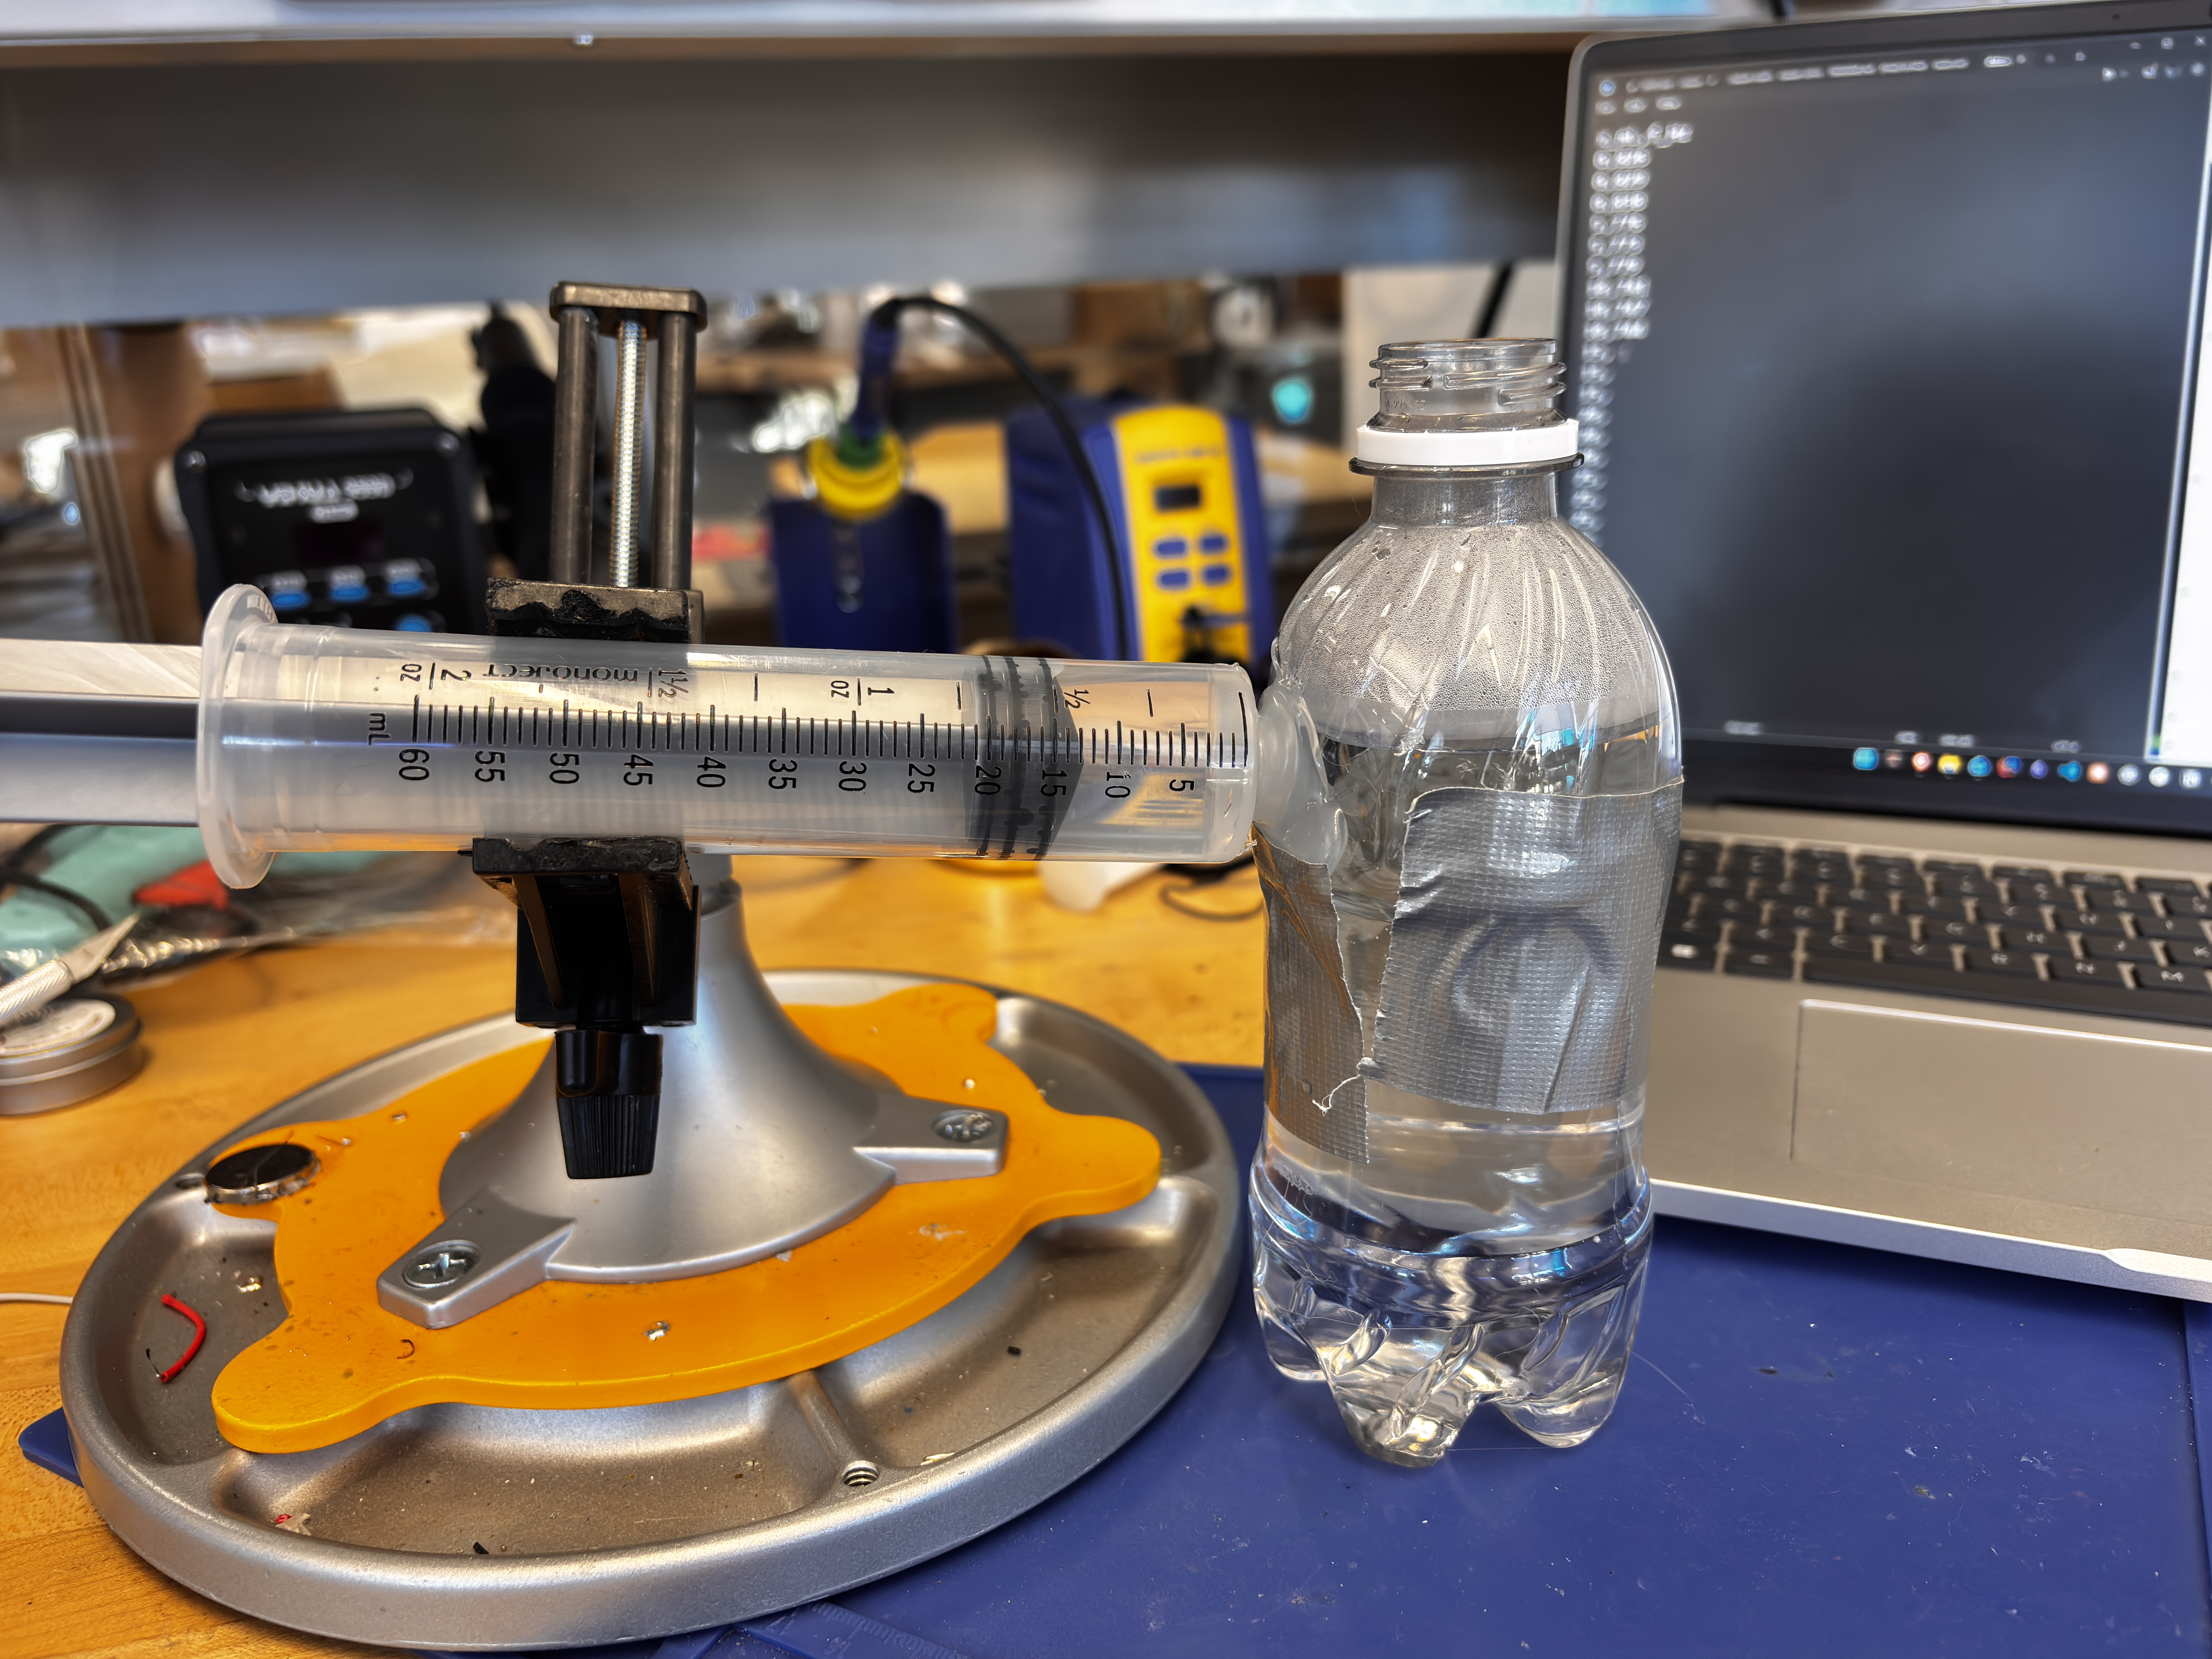
\includegraphics[width=0.78\linewidth]{device.JPG}\\
{\small\textbf{Figure 1.} The instrument set at 15 mL}
\end{center}


\section*{Raw Data}

\renewcommand{\arraystretch}{1.8}
\begin{center}
\begin{tabular}{|c|c|c|c|c|c|}
\hline
\textbf{$x$ (mL)} & \textbf{Trial 1 (Hz)} & \textbf{Trial 2 (Hz)} & \textbf{Trial 3 (Hz)} & \textbf{Mean (Hz)} & \textbf{SD (Hz)} \\
\hline
0  & 826 & 829 & 838 & 831.0 & 6.2 \\ \hline
5  & 776 & 773 & 779 & 776.0 & 3.0 \\ \hline
10 & 741 & 747 & 744 & 744.0 & 3.0 \\ \hline
15 & 712 & 709 & 709 & 710.0 & 1.7 \\ \hline
20 & 680 & 686 & 680 & 682.0 & 3.5 \\ \hline
25 & 630 & 624 & 627 & 627.0 & 3.0 \\ \hline
30 & 589 & 586 & 589 & 588.0 & 1.7 \\ \hline
\end{tabular}
\end{center}  

\newpage

%% ------------------------- Page 3: model, fit, results -------------------------
\section*{Model and Linearization}

Helmholtz resonance: $f = \dfrac{c}{2\pi}\sqrt{\dfrac{A}{V\,L_\mathrm{eff}}}$, with $V = V_0 + x$ and $L_\mathrm{eff} = L + 0.85\,d$.
Only $V$ changes, so $f = \dfrac{a}{\sqrt{V_0 + x}}$ with $a = \dfrac{c}{2\pi}\sqrt{\dfrac{A}{L_\mathrm{eff}}}\times 10^{3}$ ($x$ in mL).
Squaring and inverting linearizes it:
\[
\frac{1}{f^{2}} = \frac{1}{a^{2}}\,x + \frac{V_0}{a^{2}} ,
\]
so a least-squares line of $1/f^2$ versus $x$ has slope $1/a^2$ and intercept $V_0/a^2$, giving $a = 1/\sqrt{\text{slope}}$ and $V_0 = \text{intercept}/\text{slope}$.


\section*{Fit Results}

\renewcommand{\arraystretch}{1.6}
\begin{center}
\begin{tabular}{|l|c|c|c|}
\hline
\textbf{Quantity} & \textbf{Fitted value} & \textbf{Measured / theory value} & \textbf{Ratio (fit/theory)} \\ \hline
\multicolumn{4}{|l|}{\textit{All 7 settings ($x = 0$ to 30 mL)}} \\ \hline
slope $=1/a^2$ (Hz$^{-2}$\,mL$^{-1}$) & $4.601\times10^{-8}$ & --- & --- \\ \hline
intercept $=V_0/a^2$ (Hz$^{-2}$) & $1.379\times10^{-6}$ & --- & --- \\ \hline
$a$ (Hz\,mL$^{1/2}$) & 4662 & 5123 & 0.910 \\ \hline
$V_0$ (mL) & 30.0 & $\approx 41$ ($50 - 9$ mL neck air) & 0.73 \\ \hline
$R^2$, linearized ($1/f^2$ vs $x$) & 0.9627 & --- & --- \\ \hline
$R^2$, in $f$ vs $x$ & 0.9626 & --- & --- \\ \hline
\multicolumn{4}{|l|}{\textit{Diagnostic: same fit using only $x \le 20$ mL}} \\ \hline
$a$ (Hz\,mL$^{1/2}$) & 5381 & 5123 & 1.050 \\ \hline
$V_0$ (mL) & 42.4 & $\approx 41$ & 1.03 \\ \hline
$R^2$, linearized & 0.9940 & --- & --- \\ \hline
\end{tabular}
\end{center}

\newpage

\begin{center}
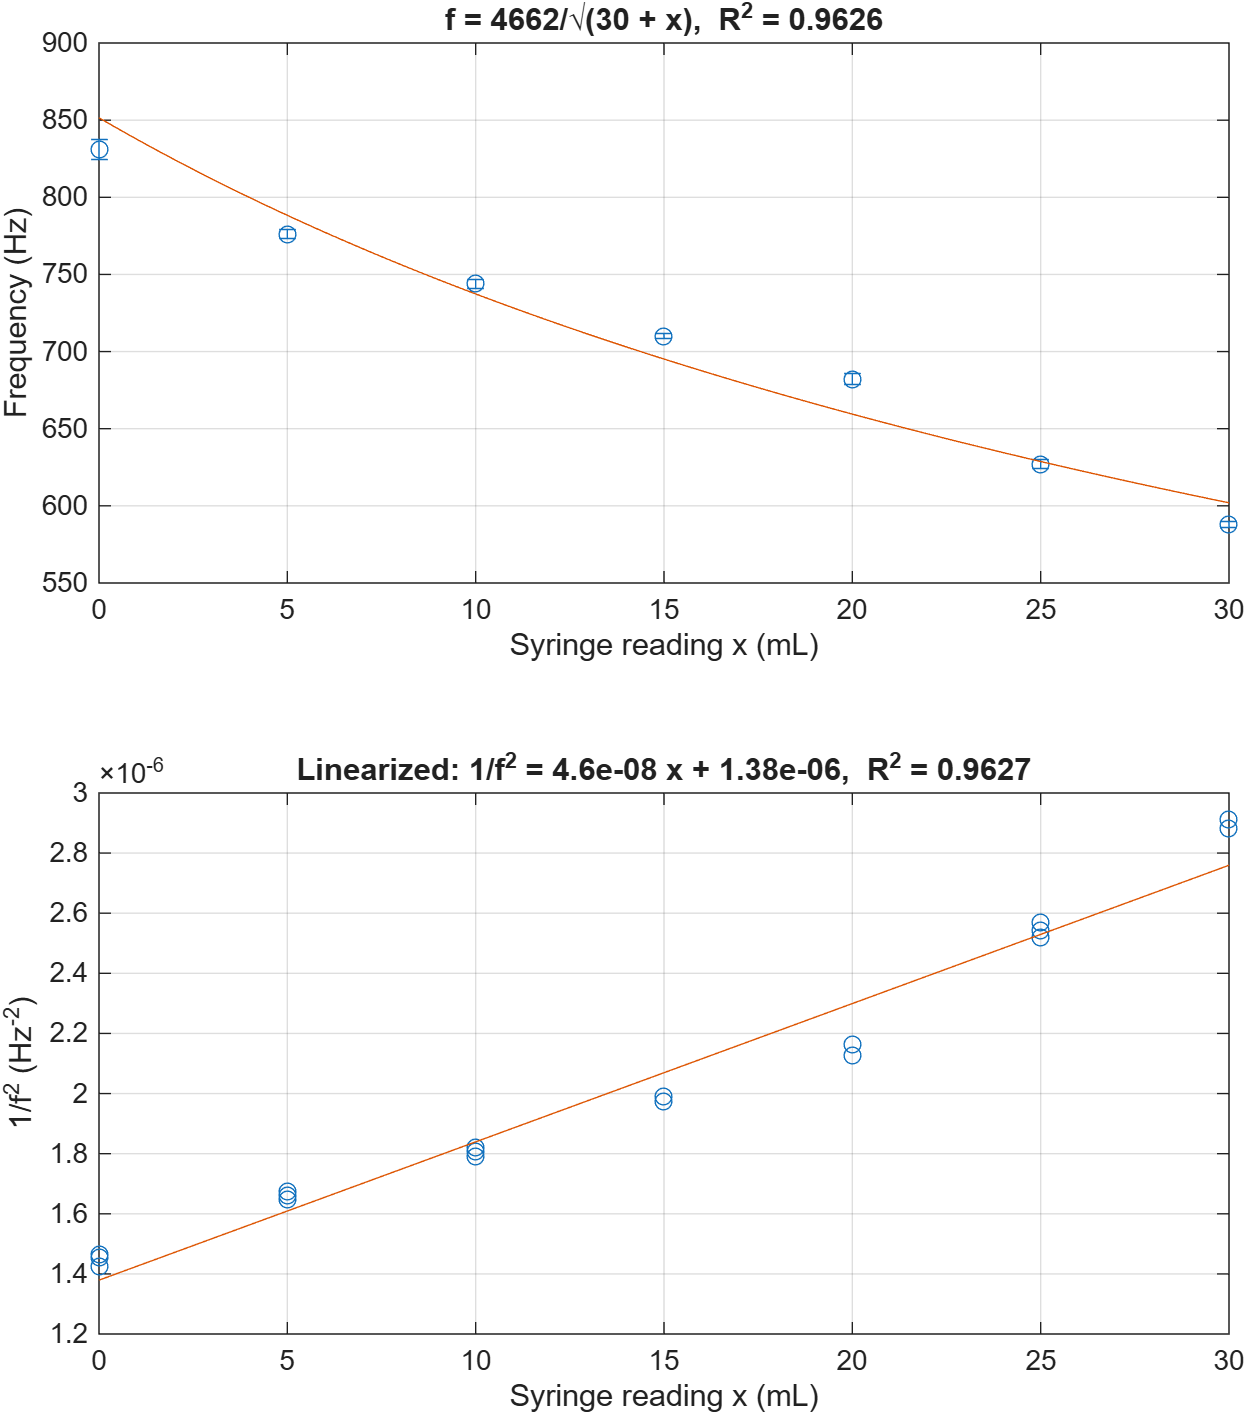
\includegraphics[width=0.78\linewidth]{plot_matlab.png}\\
{\small\textbf{Figure 1.} (Top) Fundamental frequency (Friture) vs.\ water removed $x$, mean $\pm$ SD of 3 trials at each of 7 settings,
with fit $f = a/\sqrt{V_0 + x}$, $a = 4662$, $V_0 = 30.0$ mL. (Bottom) Linearized data, $1/f^2$ vs.\ $x$, with the straight-line fit,
$R^2 = 0.9627$.}
\end{center}

\newpage

%% ------------------------- Discussion -------------------------
\section*{Discussion}
A Helmholtz-resonator bottle was built from a 355 mL Aquafina bottle (brim volume 393 mL) containing 343 mL of water, which left 50 mL of air.
When air is blown across the open neck, the plug of air in the neck is made to oscillate against the springiness of the air in the bottle, like a mass on a spring.
The note is tuned by removing water with a 60 mL syringe, which increases the enclosed air volume $V = V_0 + x$; more air gives a softer air spring and a lower pitch.


The Helmholtz resonance is given by $f = \dfrac{c}{2\pi}\sqrt{\dfrac{A}{V\,L_\mathrm{eff}}}$ with speed of sound $c$, neck area $A$, and effective neck length
$L_\mathrm{eff} = L + 0.85\,d$. Since only $V$ is changed by removing water, while $c$, $A$ and $L_\mathrm{eff}$ are held constant, $f \propto V^{-1/2}$. Equivalently, $1/f^2 = (x + V_0)/a^2$ is linear in $x$, so a straight line was fitted to $1/f^2$ versus $x$, and
$a = 1/\sqrt{\text{slope}}$ and $V_0 = \text{intercept}/\text{slope}$.

The standard deviation across three trials was 1.7--6.2 Hz (0.2--0.7\% of the frequency), and the largest scatter, 6.2 Hz, was observed at $x = 0$
where the pitch is highest. The remaining scatter is most likely caused by small changes in blowing angle and lip position and by the finite frequency resolution of the spectrum.
The measured pitch was seen to fall from 831 Hz at $x = 0$ to 588 Hz at $x = 30$ mL, a 29\% drop.

The first step, $0\to5$ mL, produced a larger change than the following steps: the pitch dropped by 55 Hz (831 to 776 Hz), compared with 28--39 Hz for most later 5 mL steps, and $1/f^2$ rose by $0.21\times10^{-6}$ Hz$^{-2}$ instead of $0.15$--$0.18\times10^{-6}$ Hz$^{-2}$. The $x=0$ point also had the largest scatter (6.2 Hz). Possible causes are that the true starting air volume differed slightly from the nominal 50 mL, since the water was added and measured by hand; that the wet neck wall and water droplets near the neck at the highest fill level changed the effective neck area slightly; and that the first draw of the syringe filled its tip, so the first reading was less reliable than later ones. Because the highest pitch (831 Hz) is also the most sensitive to blowing angle, small changes in technique may have contributed. These explanations were not tested.

The effective neck length $L_\mathrm{eff} = L + 0.85,d$ was used because the oscillating air does not stop at the physical ends of the neck: air just outside and inside the opening moves with the plug, so the plug acts longer than the neck. The factor 0.85 is the standard textbook value for two flanged ends ($\approx 0.425,d$ per end).



\vfill
\begin{center}
    \rule{0.5\linewidth}{0.5pt}\\
    \textit{End of \textbf{\hwTitle \space \hwNumber}}
\end{center}

\end{document}
